\sloppy
\documentclass[14pt,a4paper,twoside]{extarticle}	% Размер основного шрифта и формата листа
\usepackage{xltxtra}						% Используется для вывода логотипа XeLaTeX
\usepackage{xunicode}						% Кодировка документа
\usepackage{polyglossia}					% Загружает пакет многоязыковой верстки
\newfontfamily\russianfont{Book Antiqua}
%\setmainfont{Liberation Serif}						% Основной шрифт текста
\setmainfont{Book Antiqua}
\setdefaultlanguage{russian}				% Основной язык текста
\setotherlanguage{english}					% Дополнительный язык текста
\linespread{1}							% Межстрочный интервал выбран полуторным
\usepackage[left=2.5cm,
right=1.5cm,vmargin=2.5cm]{geometry} % Отступы по краям листа
\bibliographystyle{ugost2008}

\usepackage{xcolor}
\usepackage{hyperref}
% Цвета для гиперссылок
\definecolor{linkcolor}{HTML}{359B08} % цвет ссылок
\definecolor{urlcolor}{HTML}{799B03} % цвет гиперссылок
\hypersetup{pdfstartview=FitH,  linkcolor=linkcolor,urlcolor=urlcolor, colorlinks=true}

%---------------------------%
%---- Пакеты расширений ----%
%---------------------------%
\usepackage{xcolor}
\usepackage{hyperref}
% Цвета для гиперссылок
\definecolor{linkcolor}{HTML}{359B08} % цвет ссылок
\definecolor{urlcolor}{HTML}{799B03} % цвет гиперссылок
\hypersetup{pdfstartview=FitH,  linkcolor=linkcolor,urlcolor=urlcolor, colorlinks=true}


\usepackage{verbatim,indentfirst}
\usepackage{cite,enumerate,float}
\usepackage{amsmath,amssymb,amsthm,amsfonts}

%---------------------------%
%--- Вставка иллюстраций ---%
%---------------------------%
\usepackage{graphicx}
\usepackage{subfigure}
\usepackage{fontspec}
%\graphicspath{{Images/}}

\begin{document}
%\pagestyle{empty} %  выключаенм нумерацию
%\setcounter{page}{3}% Нумерация начинается с третьей страницы
%\renewcommand{\contentsname}{\center{Содержание}}
%\tableofcontents

\begin{center}
	%\addcontentsline{toc}{section}{Опыт 7. Сложение движений}
	\subsection*{Сложение движений}
\end{center}

\begin{figure}[H]
	\centering 	
	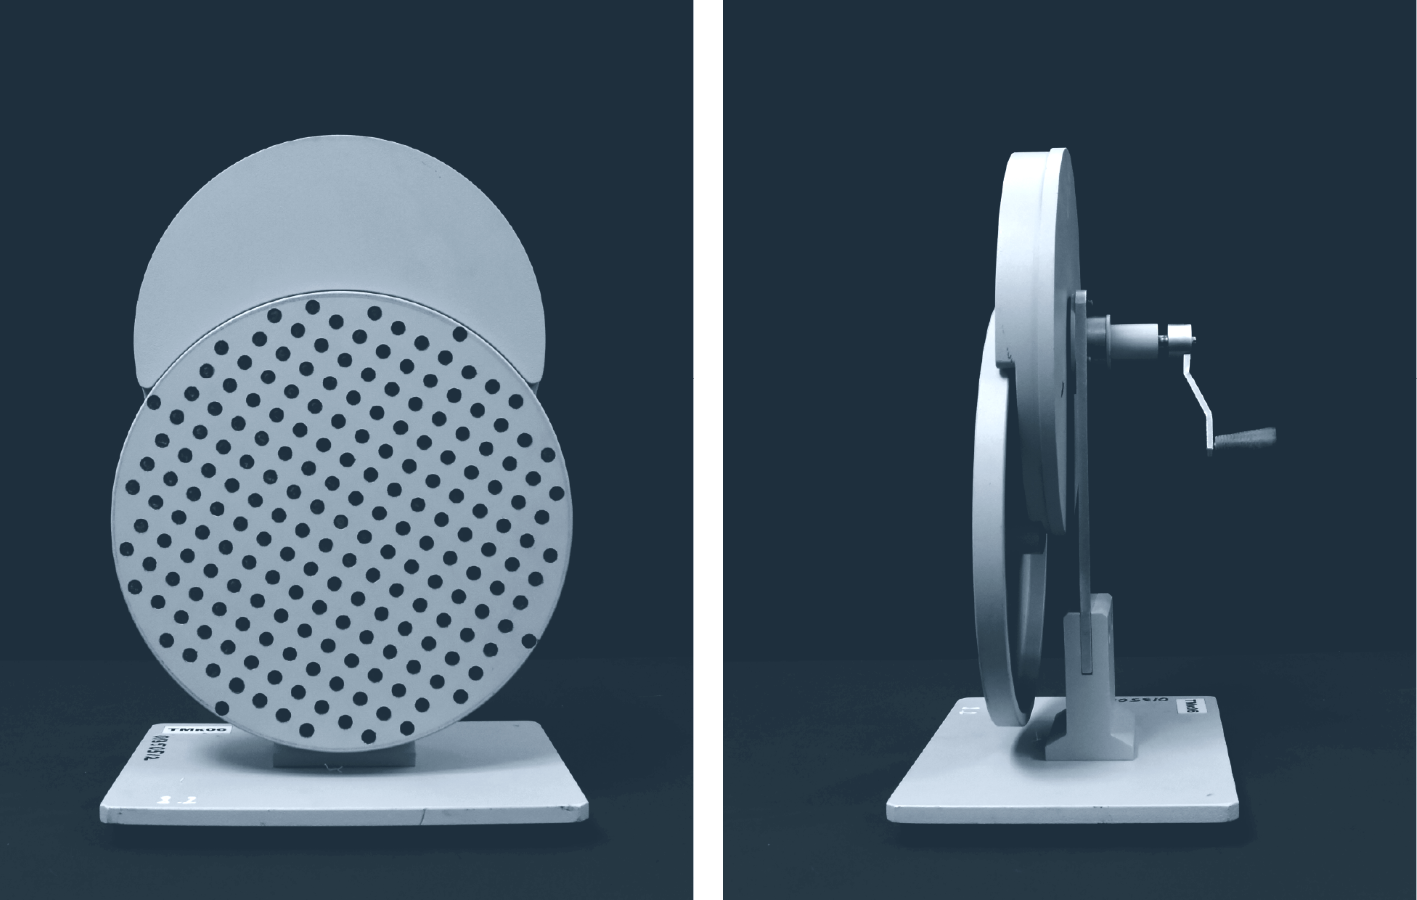
\includegraphics[width=0.9\linewidth]{aom-1.png}
	\caption{Демонстрация сложения параллельных вращений}
	\label{aom-1}
\end{figure}

\subsection*{\underline{Оборудование:}}

\begin{enumerate}
	\item Диск диаметром 26 см, поверхность которого покрыта темными кружками диаметром 1 см
	\item Подставка с механизмом, приводящим диск во вращение как вокруг его собственной оси, так и в плоскости его движения
\end{enumerate}

\newpage
\subsection*{\underline{Основные определения:}}

Вообще говоря, при движении твердого тела разные его точки 
совершают различные движения.
Но оказывается, что всегда можно 
любое такое произвольное движение тела представить как сумму 
более простых движений.
Одним из таких простых движений является поступательное движение:

\textit{\begin{flushleft}
поступательным движением называется такое движение, при 
котором любая прямая, проведенная в теле, остается параллельной 
самой себе. 
При поступательном движении все точки тела движутся одинаково. 
\end{flushleft}}

Другим простым видом движения твердого тела является вращательное движение. 
Его можно определить следующим образом: 
\textit{\begin{flushleft}
		вращательным движением называется такое движение, при ко- 
тором все точки тела движутся по концентрическим окружностям, 
а все центры этих окружностей лежат на одной прямой, называемой 
осью вращения.
\end{flushleft}}

Любое сложное движение твердого тела можно представить как сумму двух независимых 
движений: поступательного и вращательного.

\newpage
\subsection*{\underline{Краткое описание:}}

Закрепленный на подставке диск обладает горизонтальной осью вращения, проходящей через его центр.
При этом вращательный механизм способен приводить во вращение и саму ось.

Раскрутив изначально неподвижный диск вокруг собственной оси, можно наблюдать вращение темных кружков.
Удаленные от центра пятна при быстром вращении начнут сливаться в линии, а кружок в центре диска останется неподвижным (рис.\ref{aom-2}).

\begin{figure}[H] 
	\centering 	
	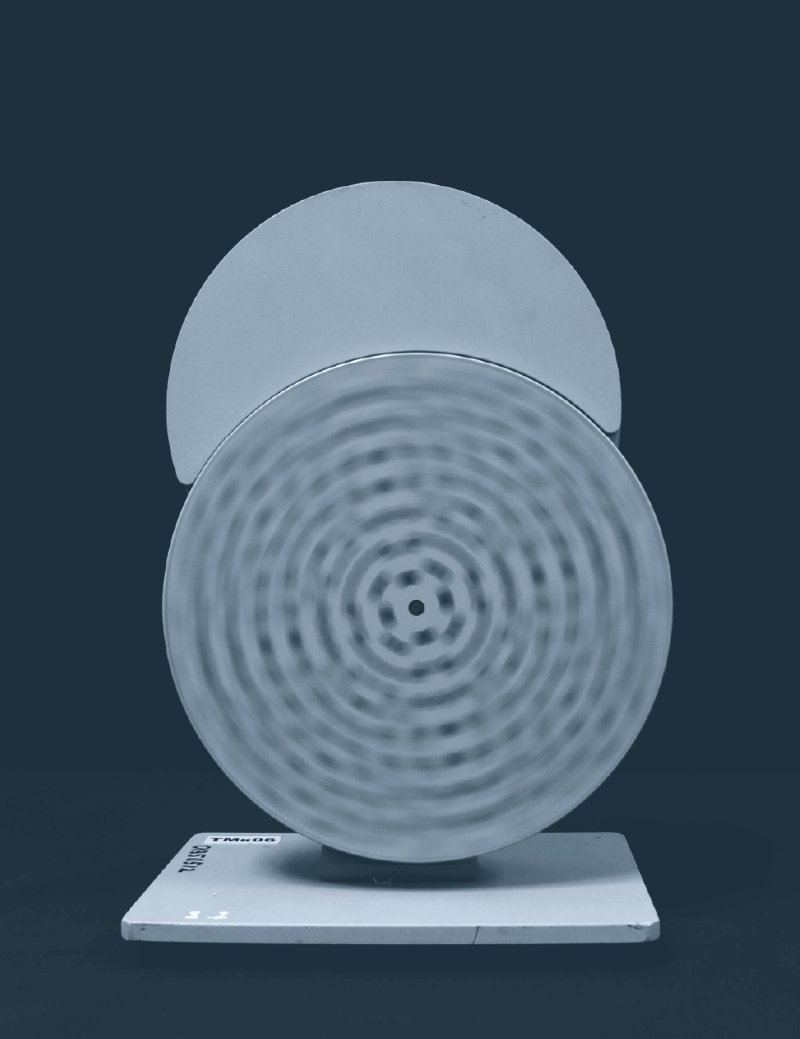
\includegraphics[width=0.6\linewidth]{aom-2.png}
	\caption{Вращение диска вокруг собственной оси, проходящей через его центр}
	\label{aom-2}
\end{figure}

Если при вращении диска его центральная ось тоже начнет описывать окружность в плоскости, параллельной диску (рис.\ref{aom-3}), то положение мгновенной оси при таком движении обнаружится по положению кружка, кажущегося неподвижным (он уже не совпадает с центром диска).

\begin{figure}[H]
	\centering 	
	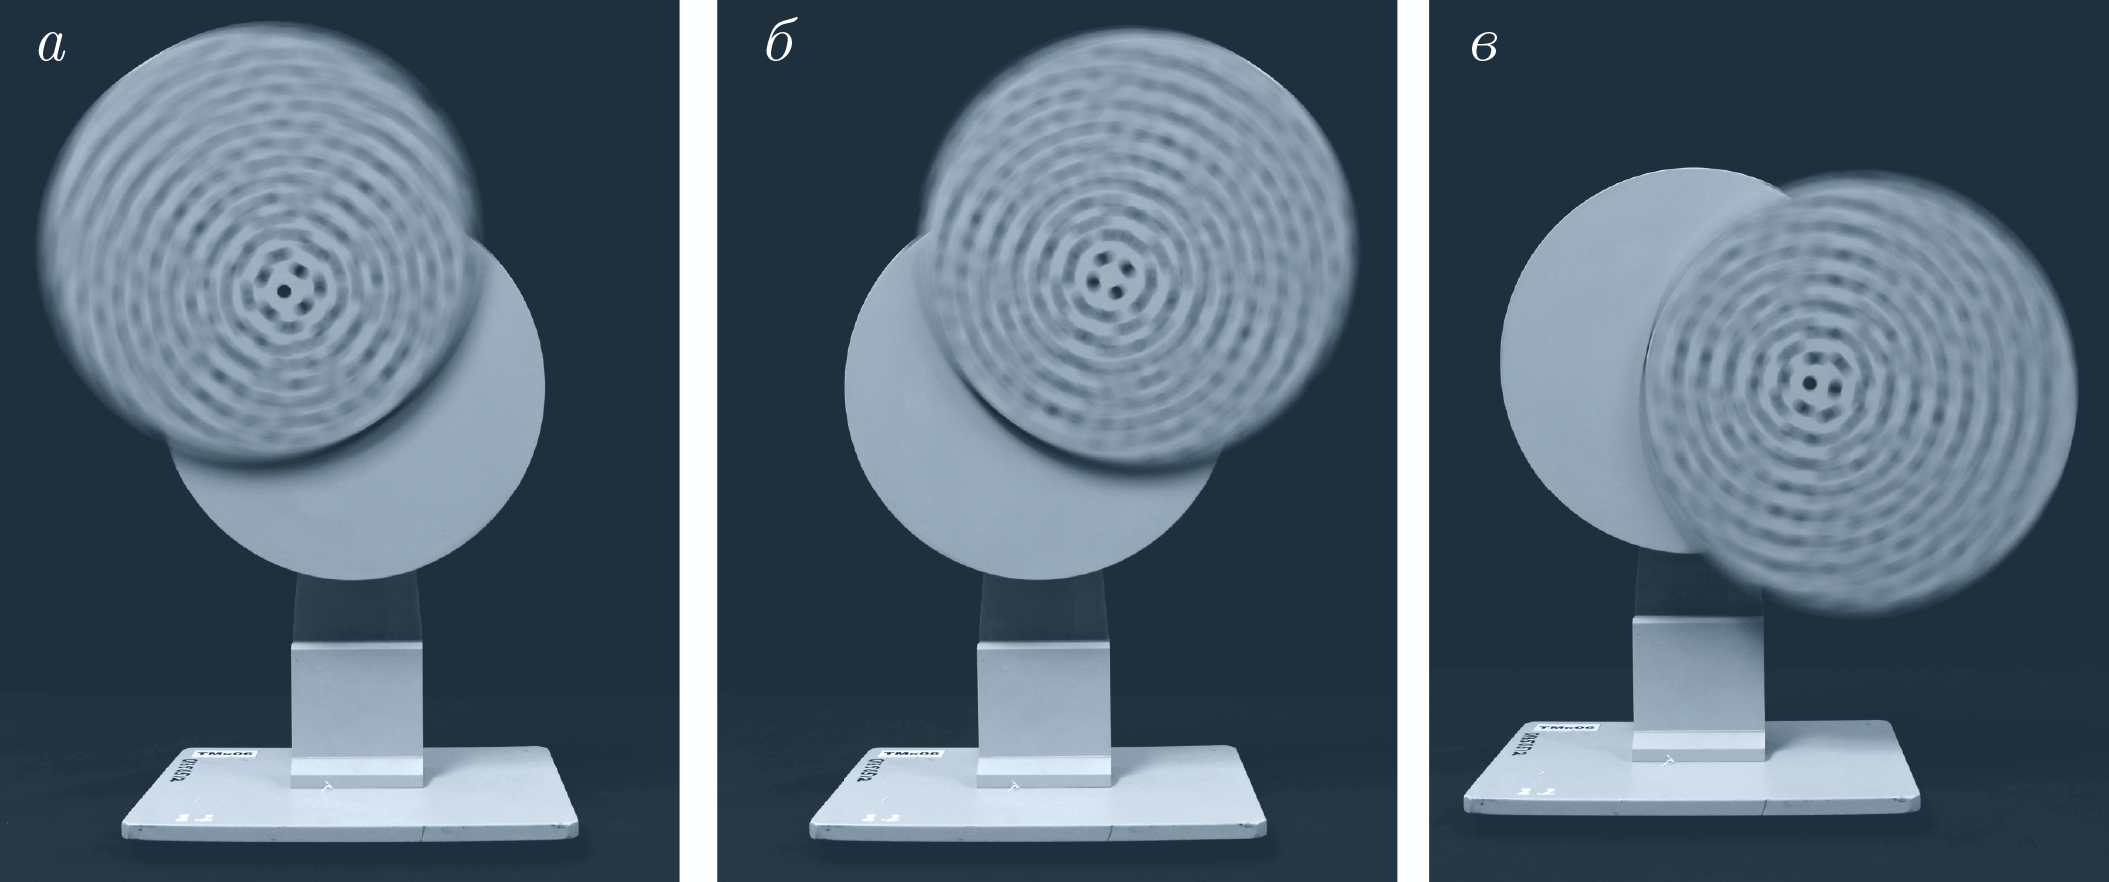
\includegraphics[width=0.9\linewidth]{aom-3.png}
	\caption{Четкое пятно находится не в центре, что связано с появлением новой — мгновенной, оси вращения. Эта ось появляется в результате того, что собственная ось тела при его вращении сама описывает окружность}
	\label{aom-3}
\end{figure}

\newpage
\subsection*{\underline{Теория:}}

Пусть диск вращается против хода часовой стрелки.
Обозначим угловую скорость его вращения через $ \textbf{ω}_1 $ (рис.\ref{aom-4},\textit{б}).

\begin{figure}[H] 
	\centering 	
	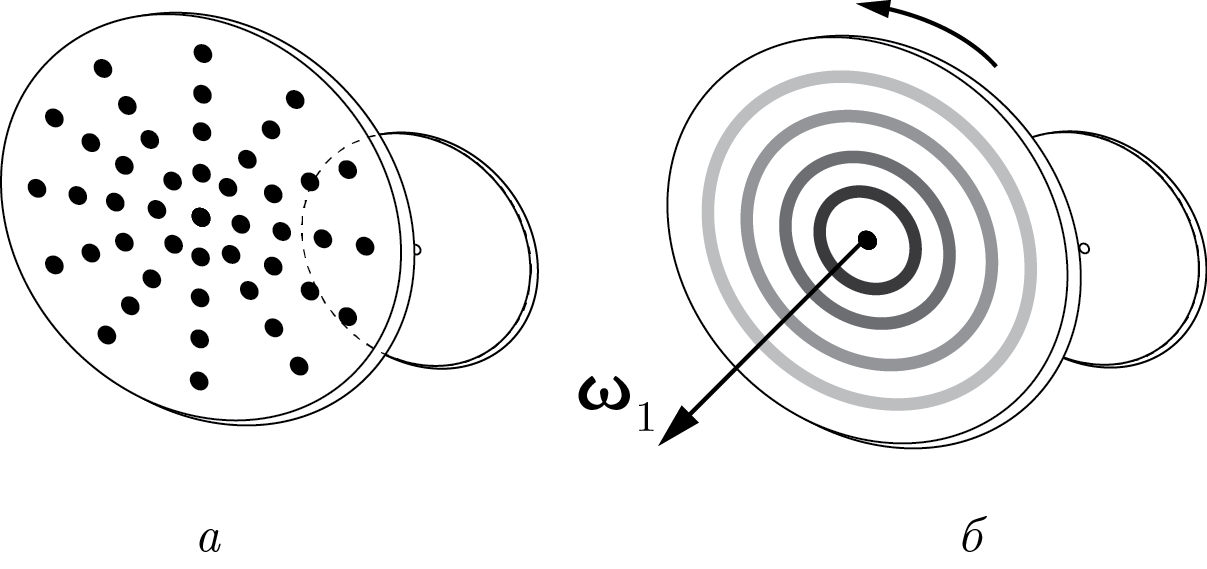
\includegraphics[width=0.75\linewidth]{aom-4.png}
	\caption{\textit{а} — схематичное изображение диска на вращающейся штативе (без вращения); \textit{б} — направление вектора угловой скорости диска при его вращении против хода часовой стрелки}
	\label{aom-4}
\end{figure}

Так как ось диска жестко связана с валом на штативе, то при одновременном вращении обоих дисков (рис.\ref{aom-5},\textit{а}) в системе появляется еще один вектор угловой скорости $ \textbf{ω}_2 $.
Результирующей скоростью вращения станет угловая скорость, равная векторной сумме скоростей диска и вала: $\textbf{ω} = \textbf{ω}_1 + \textbf{ω}_2$.

\begin{figure}[H]
	\centering 	
	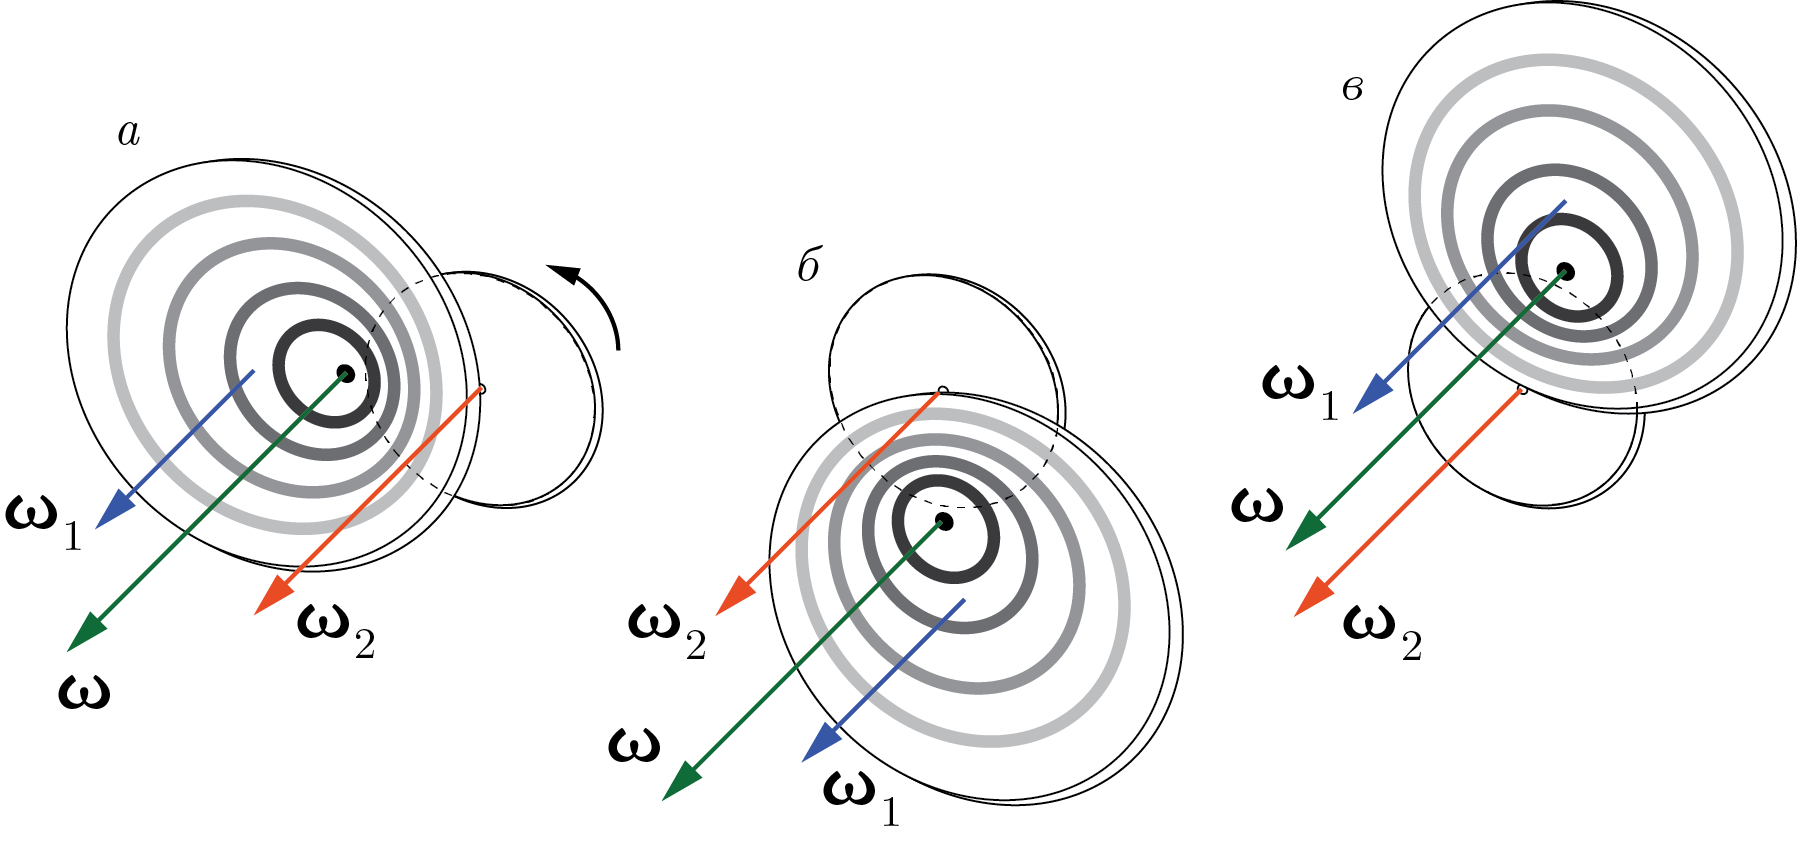
\includegraphics[width=0.9\linewidth]{aom-5.png}
	\caption{Вектор результирующей угловой скорости \textbf{ω} направлен вдоль мгновенной оси вращения, проходящей через точку на отрезке, соединяющем центры диска и вала}
	\label{aom-5}
\end{figure}

Положение мгновенной оси вращения при закручивании дисков в одну и ту же сторону (в данном случае противоположно движению часовой стрелки) можно определить через соотношение угловых скоростей:
$$
\dfrac{l_1}{l_2}  = \dfrac{\omega_2}{\omega_1}.
$$
где через $ l_1 $ и $ l_2 $ обозначены расстояния от центра диска и вала до мгновенной оси (неразмытого пятна).

\begin{figure}[H]
	\centering 	
	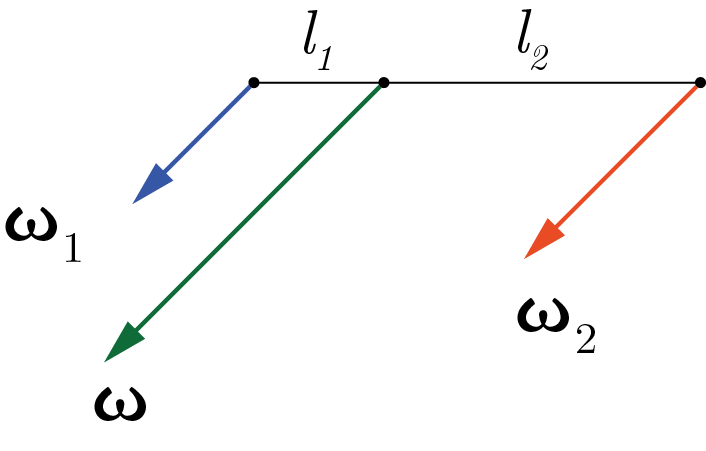
\includegraphics[width=0.3\linewidth]{aom-6.png}
	\caption{Векторы угловых скоростей диска и вала складываются, а направление результирующего вектора угловой скорости $\textbf{ω}$ совпадает с мгновенной осью вращения}
	\label{aom-6}
\end{figure}

Таким образом, по положению резкого пятна на вращающемся диске (рис.\ref{aom-3}) можно судить о соотношении угловых скоростей вращающихся тел.

\end{document}